\section{Body of the report}

This section describes the structure of different types of report and how the
text should be written. It includes tips for diagrams and equations, which are
required for most engineering reports. Finally, it addresses the vital topic of
references and how you should acknowledge the work of others.

\subsection{Structure and sections}

The structure of the report and the titles of sections depend on the nature of
the project. Here are suggestions for two extreme types, which can be adjusted
to suit your report.

\subsubsection{Research projects}

Here you are given a starting point and a general direction: your aim is to
discover something new. The report would probably be divided into sections with
familiar titles.

\begin{itemize}
    \item \textbf{Theory} {--} Explain essential background theory that is vital
          for the reader to understand your report. Select and present the
          material to show its relevance to the project and demonstrate your
          understanding. Do not repeat standard material from textbooks, which
          is a waste of space; give a reference instead. This section should
          lead into the Objectives of your project: the specific questions that
          your research will address.
    \item \textbf{Experimental Techniques} {--} Give an account of your
          experimental or numerical techniques. Emphasise details that would be
          necessary to continue the work or to compare your results with those
          of other experimenters. Include what you would have liked to know at
          the start of your project but don’t copy material from manuals or
          other references.
    \item \textbf{Results} {--} Describe these at an appropriate level of detail to
          support your conclusions. Be selective: you cannot include everything.
          Lengthy tables should be left to an appendix. Avoid unnecessary
          detail: describe preliminary experiments briefly if at all, unless
          they illustrate some important point.
\end{itemize}

\subsubsection{Design, build and test projects}

Here the goal is specified, more or less precisely: your job is to work out how
to get there. The titles of the sections are less standardised but here is a
possible approach.

\begin{itemize}
    \item \textbf{Specification} {--} Typically you are given only a vague
          description of the functions required as the aims and must first
          develop this into a firm specification against which your final
          product will be judged. This may be a fairly long section because you
          need to justify your choices. The detailed specification provides the
          objectives for this type of project.
    \item \textbf{Possible strategies} {--} Evaluate briefly the possible
          approaches that you considered and explain why you selected one of
          these. Avoid excessive detail of discarded possibilities.
    \item \textbf{Implementation} {--} Describe the final product. Concentrate
          on key features that required advanced design and skim over well-known
          aspects. Mention useful points that might help future students, such
          as tricky sections of data sheets.
    \item \textbf{Testing} {--} This is equivalent to the ‘Results’ section of a
          research project.
\end{itemize}

\subsection{Style of writing}

One of the most difficult aspects of writing is to judge the level and
background of your readers. Typically the report is assessed by your first
supervisor, who is an expert on the topic, and your second supervisor, who is
not. You should therefore assume that the reader is a \textit{well-educated,
    graduate engineer} but not an expert on the subject of the project. Assume that
he or she is familiar with the general concepts taught in courses up to level 3
but not with the details of specialised courses at higher levels.

It is also difficult to appreciate that most readers are not interested in the
nitty-gritty detail. They want to know \textit{what} you did and \textit{why}
you did it that way but they don’t want a step-by-step account of \textit{how}
you did it. Your watchword should therefore be:

\begin{center}
    \large\textbf{SUMMARISE!}
\end{center}

Of course some people need the details {--} a person continuing work on the
project requires precise experimental methods, for instance. Such material is
best in an appendix. The same is true for computer programs and schematics of
complicated circuits. Design-and-build projects may need a User’s Manual, which
should be included as an appendix.

A report is a formal document and should be written in appropriate language.
Numerous books offer advice on writing reports and a selection [1, 2, 3, 4] is
listed in the references at the end. Here are a few tips.

\begin{itemize}
    \item Reports should be written in correct English. Break text into
          paragraphs, keep sentences to a reasonable length and insert
          appropriate punctuation. Use a spell-checker and a grammar-checker if
          desired but neither is a substitute for careful reading.
    \item A report is not a story. Write ‘The voltage was measured’ rather than
          ‘I measured the voltage’. This document contains instructions and
          therefore uses a different style.
    \item Define all abbreviations when they are first used: ‘The accelerometer
          uses a serial peripheral interface (\gls{spi})’. Provide a list of
          abbreviations if you use a large number of them.
    \item Don’t write material that you don’t understand. It will be obvious to
          the reader.
\end{itemize}

\subsection{Precision}

An engineering report must be precise. This applies both to the language and to
numerical values. For example, the words precision and accuracy are often used
interchangeably in non-technical discussion but the distinction between them is
vital in engineering. Vague, waffly text is a major weakness of many students’
technical reports (and examination answers).

Quote numerical results to an appropriate number of significant figures. For
example, it is pointless to claim that a length was 12.345 mm if it was measured
with a pocket ruler. Don’t simply write down all the digits displayed on your
calculator.

Analyse the uncertainties in your results to increase the impact of your
results. Please avoid horrors like this:

\begin{displayquote}
    The gain was quite accurate.
\end{displayquote}

The sentence is meaningless and the reader will doubt whether you have any idea
of the accuracy. Contrast this sentence:

\begin{displayquote}
    The accuracy of the gain was estimated to be \(\pm2\%\), limited by the
    tolerance of the resistors. A detailed analysis is given in Appendix C.
\end{displayquote}

This is informative and convinces the reader that you have a full understanding.

\begin{figure}[htb]
    \centering{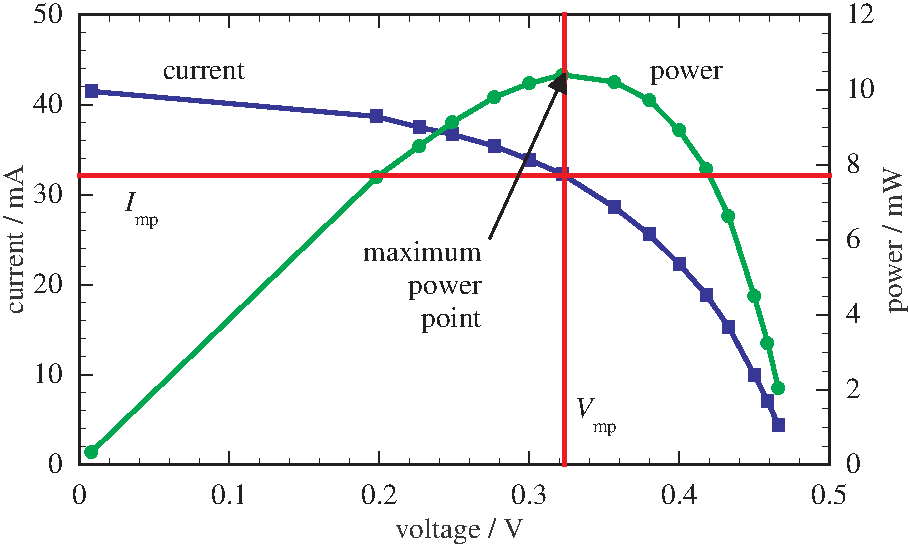
\includegraphics[width=0.7\textwidth]{Figures/solarcell.pdf}}
    \caption[Current and Power as A Function of Voltage Delivered by A Single
        Photovoltaic Cell]{Current and power as a function of voltage delivered by a
        single photovoltaic cell: under illumination from a 150 W metal halide
        floodlamp, showing the maximum power point.}\label{f:solarcell}
\end{figure}

\subsection{Figures and tables}

Figures (diagrams, photographs etc) and tables must have informative captions
and be numbered as in \autoref{f:solarcell}. Axes of graphs should have scales,
titles and units, otherwise the plot is meaningless. Multiple curves must be
labelled, either directly as in \autoref{f:solarcell} or with a caption. Use
dotted or dashed lines as well as colour for clarity; remember that the reader
might be colour-blind or have only a black-and-white printout. All text must be
legible, roughly the same size as the main text. Be warned that plots from Excel
or Matlab need extensive editing to bring them up to an acceptable standard.
Experimental traces can be captured on most modern test equipment and can make
good illustrations.

Never use screenshots or images taken with a camera where a more professional
method is available.

Be careful if you paste figures into Microsoft products, which seem to wreck
almost any format; png files may be best. Do not distort the image by changing
the aspect ratio (width:height).

Tables must have appropriate headings with units. Avoid lengthy tables: consider
whether a graph would be clearer or the data would be better in an appendix.

\subsection{Equations}

Most engineering reports contain equations. Do not type these as though they are
ordinary text in Word but use an equation editor. Short equations, such as
\(ax^2+bx+c=0\), can be written inline but longer equations should be displayed
like this:

\begin{equation}
    x=\frac{-b\pm\sqrt{b^2-4ac}}{2a}
\end{equation}

Number equations so that you can refer to them. Consider \LaTeX{} if you have a
lot of mathematics.

\subsection{Software}

It is tricky to describe software well. Often the best approach is to describe
the high-level structure in the main text (a UML diagram for example) and pick
out any special features of the program that need to be explained in detail. A
complete listing should be included as an appendix. Do not describe your
complete code line by line; you will send the reader to sleep. Please make sure
that the listing is formatted to make it easy to read and understand;
screenshots are unacceptable.

You must supply references to make it clear where your computer code includes
material from elsewhere, such as published libraries or code examples. This is a
perfectly acceptable approach (it is why the material is made available) but you
must:

\begin{itemize}
    \item provide a reference to the source of the material
    \item use comments in the listings to make it absolutely clear which parts
          were written by you and which were taken from published material.
\end{itemize}

If you do not do this, the reader will assume that the code is all your own work
and you will be guilty of plagiarism if this is not correct. See the next
section.

\subsection{References}

No project is done in isolation. A research project builds on the results of
previous workers; a design-and-build project depends on the properties of the
components available. You therefore draw on published documents during your
project and must provide references to these sources in your report. References
are cited (a) to give due credit to the originator and (b) to guide a reader who
wants more detailed information. You should give a reference wherever it is
required for either of these purposes. Properly referenced material from many
sources is a sign of a good project report.

References must be cited with sequential numbers in square brackets where they
are used in the text. Typical usage is `Fitzmaurice and Hand
\autocite{fitzmaurice1987comparison} showed that\ldots’ or `The median is an
appropriate estimator for this signal \autocite{fitzmaurice1987comparison}'

Avoid direct quotations from references in general; make it absolutely clear
that the text is a quotation if this is unavoidable. An illustration, such as a
diagram from a data sheet, is another type of quotation and must be referenced,
typically in the figure caption. This is perfectly acceptable: do not waste time
redrawing diagrams.

\subsubsection{Plagiarism}

If you copy from another person’s work (project report, book, journal, code, web
page or any other document) without acknowledging the source, you are guilty of
plagiarism. This is a disciplinary offence and the University has procedures for
handling it. The failure to acknowledge a source is considered as plagiarism
even if there was no deliberate intention to cheat.

Avoid any risk of plagiarism by providing a reference for all sources that you
use. Read the advice offered by the University at
\url{www.gla.ac.uk/services/sls/plagiarism} and consult your supervisor if you
are in any doubt. The University’s
\href{http://www.gla.ac.uk/services/senateoffice/studentcodes/staff/plagiarism/plagiarismstatement/}{Plagiarism
    Statement} is reproduced in \autoref{s:plagiarism}.

All project reports are submitted to \href{http://www.submit.ac.uk/}{Turnitin}
or another application that checks for originality as part of the university’s
policy \textquote{to provide a means whereby students may enhance their
    knowledge and understanding of plagiarism}'. The policy also states that
\textquote{students must always be allowed the opportunity to run a draft of
    their assignment through the originality check system to gain feedback before
    being asked to submit a final document}. The checker highlights your text to
show material that is similar to other documents in its database. Some phrases
are so common that they are always highlighted and this is no cause for concern.
However, we will look more closely if whole sentences or larger blocks of text
are highlighted.

The overall fraction of highlighted material is shown as a similarity
percentage. The most common question from students is \textquote{What similarity
    percentage is acceptable?} A quick answer is 10\% but it is meaningless for the
following reasons.

\begin{itemize}
    \item It may be appropriate for you to quote a large block of text in your
          report. For example, you might be developing a product to meet an
          unusual design code and feel that the reader must know the details of
          this code to understand why you approached your project in a
          particular way. Turnitin will highlight the design code but this is
          acceptable provided that you have referenced it correctly, even if it
          is more than 10\% of your report. (Please consider whether this is the
          best approach, though.)
    \item If you have copied material into your results, analysis or
          conclusions, it will almost certainly be treated as serious plagiarism
          even if it is less than 1\% of your report. You may be expelled from
          the university for such an offence.
\end{itemize}

An automatic checker is not the only method used to detect plagiarism. Some
sources are not included in its database but your supervisor knows the
literature well. Images can be plagiarised in the same way as text.

\subsubsection{List of references}

All reports must have a section entitled References after the main text but
before any appendices. This comprises a list of sources, numbered to match the
citations in the text. Each reference requires the following information and the
cited references provide examples.

\begin{itemize}
    \item Journal paper {–-} author(s), title of paper, name of journal, volume
          number, first page, last page and year
          \autocite{fitzmaurice1987comparison}. Many journals now use article
          numbers instead of page numbers.
    \item Book {--} author(s), title, edition, publisher and year of publication
          \autocite{van2017writing}. Include the number of the chapter or
          page(s) if you refer to only a small part of the book.
    \item Data sheet {--} company, title, edition, URL and date
          \autocite{datasheet}. Application notes, technical reports and similar
          documents should be cited in the same way.
    \item Web page {--} author(s) or organisation, title, full URL and date of
          viewing \autocite{oxford}. See below.
\end{itemize}

The reader must be able to find the document without further searching.

\subsubsection{References from the Web}

The World Wide Web is a wonderful resource because it is so easy to search. It
is therefore tempting to use web pages as references. Proceed with caution
because the accuracy of many web sites cannot be verified. This is particularly
true for anonymous sites such as Wikipedia. Use them only as a starting point:
good pages provide references to more authoritative sources.

Reports whose references are all or mainly from the web, especially from
anonymous sites, will be penalised.